

\glssetexpandfield{desc} %Comando para expandir otros comandos en la descripcion de los glosarios
\glssetexpandfield{name} %Comando para expandir otros comandos en el nombre de los glosarios
%==========================CONTADORES==============================%
%Se crea nuevo contador que se utiliza para agregar las letras correspondientes a los anexos
\newcounter{anexosletra}

%Se establece 1 como el valor inicial del contador
\setcounter{anexosletra}{1}

%Se crea el contador que se utiliza para agregar el numero correlativo de las secciones dentro de un anexo
\newcounter{anexosseccion}

%Se crea el contador que se utiliza para agregar el numero correlativo de una subseccion dentro de un anexo
\newcounter{anexossubseccion}

%Se crea el contador que se utiliza para llevar la cuenta de cuantos autores han sido ingresados en la primera portada, esto sirve para saber si la mayoria son hombres o mujeres y tambien para establecer un maximo de cuatro autores
\newcounter{contadorautor}

%Se establece el valor inicial 0 para el contador de autores
\setcounter{contadorautor}{0}

%Se crea el contador que se utiliza para llevar la cuenta de cuantos autores son hombres
\newcounter{contadorhombres}

%Se establece el valor inicial 0 para el contador de hombres
\setcounter{contadorhombres}{0}

%Se crea el contador que se utiliza para llevar la cuenta de cuantos autores son mujeres
\newcounter{contadormujeres}

%Se establece el valor inicial 0 para el contador de mujeres
\setcounter{contadormujeres}{0}

%
\newcounter{resultadosexosautores}
\setcounter{resultadosexosautores}{0}

\newcounter{figuras}
\setcounter{figuras}{0}

%===========================COMANDOS=============================%

%Este comando verifica que el parametro que le pasaron este vacio o no
\newcommand{\verificarvacio}[3]{
    \ifdefined #1
        \ifthenelse{\equal{#1}{}}{%
        %Si esta vacio muestra un mensaje de advertencia en mayuscula y de color rojo
        \textcolor{red}{\MakeUppercase{#2}}%
        }{
        %Si no esta vacio entonces muestra el texto del parametro en mayuscula
        \MakeUppercase{#1}
        }
    \else
        \textcolor{red}{\MakeUppercase{#3}}
    \fi
}

% Estos comandos guardan los nombres de los integrantes del grupo, el comando autorA corresponde al primer autor, autorB corresponse al segundo autor, autorC corresponde al tercer autor y autorD corresponde al cuarto autor
\newcommand{\autorA}{}
\newcommand{\autorB}{}
\newcommand{\autorC}{}
\newcommand{\autorD}{}

%El comando autor se encarga de agregar los nombres de los autores en los comandos anteriores
\newcommand{\autor}[2]{
    %Se verifica cuantas veces se a utilizado el comando autor, si se ha hecho menos de cuatro veces entonces todavia se pueden agregar mas autores, si se ha hecho igual o mas de cuatro veces entonces ya no se puede agregar mas autores
    \ifthenelse{\value{contadorautor} < 4}{
        %El contador "contadorautor" sirve para llevar la cuenta de cuantos autores se han ingresado, el comando \ifcase sirve para verificar que valor tiene el contador en ese momento y en base a eso hacer una acción u otra.
        \ifcase\value{contadorautor}%
            %Si el contador es 0 no se ha ingresado ningun autor todavia, por lo tanto se agrega el nombre al comando autorA
            \renewcommand{\autorA}{#1}
        \or%
            %Si el contador es 1 se ha ingresado ya un autor, por lo tanto se agrega el nombre al comando autorB
            \renewcommand{\autorB}{#1}
        \or%
            %Si el contador es 2 se han ingresado dos autores, por lo tanto se agrega el nombre al comando autorC
            \renewcommand{\autorC}{#1}
        \or%
            %Si el contador es 3 se han ingresado tres autores, por lo tanto se agrega el nombre al comando autorD
            \renewcommand{\autorD}{#1}
        \fi

        %Se valida que el sexo ingresado para cada un autor sea hombre o mujer, si es mujer el contador "contadormujeres" incrementa en 1, si en hombre el contador "contadorhombres incrementa en 1
        \ifthenelse{\equal{#2}{M}}{
            \stepcounter{contadormujeres}
        }{
            \stepcounter{contadorhombres}
        }

        %Se incrementa en 1 el contador "contadorautor" al final del comando
        \stepcounter{contadorautor}
    }{
    
    }
}

%Este comando sirve para verificar el numero de mujeres y hombres en el grupo de trabajo ya que es necesario para escribir el grado a optar en la primera portada del trabajo
\newcommand{\verificarsexoautores}{
    \ifthenelse{\equal{\value{contadormujeres}}{0}}{
        %Si no hay mujeres en el grupo entonces el valor del contador resultadosexosautores es 1
        \setcounter{resultadosexosautores}{1}
    }{
        \ifthenelse{\equal{\value{contadorhombres}}{0}}{
            %Si no hay hombres en el grupo entonces el valor del contador resultadosexosautores es 2
            \setcounter{resultadosexosautores}{2}
        }{
            \ifthenelse{\value{contadorhombres} > \value{contadormujeres} }{
                %Si hay mas hombres que mujeres entonces el valor de resultadosexosautores es 3
                \setcounter{resultadosexosautores}{3}
            }{
                \ifthenelse{\value{contadormujeres} > \value{contadorhombres}}{
                    %Si hay mas mujeres que hombres entonces el valor de resultadosexosautores es 4
                    \setcounter{resultadosexosautores}{4}
                }{
                    \ifthenelse{\equal{\value{contadorhombres}}{\value{contadormujeres}}}{
                        %Si hay igual numero de mujeres que de hombres el valor del contadore resultadosexosautores es 5
                        \setcounter{resultadosexosautores}{5}
                    }{
                    
                    }
                }
            }
        }
    }
}

%Valor booleano para saber si ya se ingreso alguna entrada a las siglas o no
\newcommand{\ningunasiglaingresada}{true} 

%Este comando sirve para agregar nuevas siglas a la seccion de siglas
\newcommand{\itemsiglas}[2]{%
    %Valida que se agreguen entradas a las siglas solo si los dos parametros del comando \itemsiglas han sido llenados, si no han sido llenados no se agreaga ninguna sigla nueva
    \ifthenelse{\equal{#1}{} \or \equal{#2}{}}{ 
    
    }{
    %Si los dos parametros fueron agregados entonces se ingresa la nueva sigla y \ningunasiglaingresada cambia a falso
        \renewcommand{\ningunasiglaingresada}{false}
        \newglossaryentry{#1}{name={#1}, type=siglas, description={#2}}%
    }
}

%Valor booleano para saber si ya se ingreso alguna entrada a las abreviaturas o no
\newcommand{\ningunaabreviaturaingresada}{true} 

%Este comando sirve para agregar nuevas abreviaturas a la sección de abreviaturas
\newcommand{\itemabreviatura}[2]{
    %Valida que se agreguen entradas a las abreviaturas solo silos dos parametros del comando \itemabreviatura han sido llenados, si no han sido llenados no se agreaga ninguna abreviatura nueva
    \ifthenelse{\equal{#1}{} \or \equal{#2}{}}{  
    }{
    %Si los dos parametros fueron agregados entonces se ingresa la nueva abreviatura y \ningunaabreviaturaingresada cambia a falso
        \renewcommand{\ningunaabreviaturaingresada}{false}
        \newglossaryentry{#1}{name={#1}, type=abreviaturas, description={#2}}%
    }
    
}

%Valor booleano para saber si ya se ingreso alguna entrada a la nomenclatura o no
\newcommand{\ningunanomenclaturaingresada}{true}

%Este comando sirve para agregar un nuevo elemento a la sección de nomenclatura
\newcommand{\itemnomenclatura}[2]{%
    %Valida que se agreguen entradas a la nomenclatura solo silos dos parametros del comando \itemnomenclatura han sido llenados, si no han sido llenados no se agreaga ninguna nomenclatura nueva
    \ifthenelse{\equal{#1}{} \or \equal{#2}{}}{       
    }{
    %Si los dos parametros fueron agregados entonces se ingresa la nueva nomenclatura y \ningunanomenclaturaingresada cambia a falso
        \renewcommand{\ningunanomenclaturaingresada}{false}
        \newglossaryentry{#2}{name={#1}, type=nomenclatura, description={#2}}%
    }
}

%Valor booleano para saber si ya se ingreso alguna entrada al glosario o no
\newcommand{\glosariovacio}{true} 

%Este comando sirve para agregar nuevas palabras al glosario
\newcommand{\itemglosario}[2]{%
    %Valida que se agreguen entradas al glosario solo si los dos parametros del comando \glosario han sido llenados, si no han sido llenados no se agreaga ninguna entrada al glosario nueva
    \ifthenelse{\equal{#1}{} \or \equal{#2}{}}{ 
        
    }{
    %Si los dos parametros fueron agregados entonces se ingresa la nueva
    %entrada del glosario y \glosariovacio cambia a falso
        \renewcommand{\glosariovacio}{false}
        \newglossaryentry{#1}{name={#1}, type=glosario, description={#2}}%
    }
}


%Este comando esta creado para hacer uno o dos saltos de pagina dependiendo de si la seccion termina en pagina impar o par
\newcommand{\paroimpar}[1]{
    \pgfmathparse{mod(#1,2)}
    \edef\resultado{\pgfmathresult}% Almacenar el resultado como una macro expandida

    \ifthenelse{\equal{\resultado}{0.0}}{
        \newpage
    }{
        \newpage
        \null\thispagestyle{empty}
        \newpage
    }
}

%Comando utilizado para crear los capitulos
\newcommand{\capitulo}[2]{
    \begin{capituloentorno}
    {
        #1
    }{
        #2
    }
    \end{capituloentorno}
}

%Valor booleano para saber si ya se agrego una imagen al documento o no
\newcommand{\ningunaimageningresada}{true}

% Se crea nuevo comando que establece el formato de las figuras
\newcommand{\imagen}[6]{
    \renewcommand{\ningunaimageningresada}{false}
    %Se valida si existe alguna imagen con el nombre proporcionado
    \IfFileExists{img/#1}{
        %Se cambia el valor del comando ningunaimageningresada a false
        \renewcommand{\ningunaimageningresada}{false}
        %\stepcounter{figuras}
        %Si el cuarto parametro del comando es V significa que se quiere mostrar la imagen en formato vertical.
        \ifthenelse{\equal{#6}{V}}{
            %Se valida que el tercer parametro no este vacio, el tercer parametro corresponde a la escala que tendra la figura, si el parametro esta vacío entonces se coloca 1 por defecto
            \ifthenelse{\equal{#5}{}}{
                \begin{figure}[H]
                \vspace{2\baselineskip}
                \centering
                \includegraphics[scale=1]{img/#1}
                \ifthenelse{\equal{#3}{true}}{
                    \caption[#2]{#2. Adaptado de: [#4]}
                }{
                    \caption[#2]{#2. Fuente: [#4]}
                }
                \label{fig:#1}
                \end{figure}
            }{
            %Si no esta vacio entonces se coloca el valor que se escribio en el tercer parametro
                \begin{figure}[H]
                \vspace{2\baselineskip}
                \centering
                \includegraphics[scale=#5]{img/#1}
                \ifthenelse{\equal{#3}{true}}{
                    \caption[#2]{#2. Adaptado de: [#4]}
                }{
                    \caption[#2]{#2. Fuente: [#4]}
                }
                \label{fig:#1}
                \end{figure}
            }    
        }{
        %Si el cuarto parametro es H significa que la figura se mostrara de manera horizontal
        \ifthenelse{\equal{#6}{H}}{
            \begin{sidewaysfigure}
                \includegraphics[width=\linewidth]{img/#1}
                \ifthenelse{\equal{#3}{true}}{
                    \caption[#2]{#2. Adaptado de: [#4]}
                }{
                    \caption[#2]{#2. Fuente: [#4]}
                }
                \label{fig:#1}
            \end{sidewaysfigure}
        }{
        \textcolor{red}{\MakeUppercase{ERROR: el parametro para la orientacion de la imagen solo puede ser 'H' para horizontal y 'V' para vertical}}
        }
        }
    }{
        \textcolor{red}{\MakeUppercase{ERROR: la imagen con nombre #1 no existe}}
    }
}

%Este comando sirve para escribir la carrera que se esta cursando de la manera correcta en la primera porta validando la cantidad de mujeres y hombres en el grupo
\newcommand{\determinarcarrera}[2]{
    %Si el segundo parametro del comando es 1 significa que se inserata el nombre de la carrera en la segunda portada en la parte del director de carera
    \ifthenelse{\equal{#2}{1}}{%
        %El primer parametro indica la carrera que se esta cursando
        \ifcase #1%
            INGENIERÍA INFORMÁTICA%
        \or%
            INGENIERÍA CIVIL%
        \or%
            INGENIERÍA ELÉCTRICA%
        \or%
            INGENIERÍA ENERGÉTICA%
        \or%
            INGENIERÍA DE ALIMENTOS%
        \or%
            INGENIERÍA QUÍMICA%
        \or%
            INGENIERÍA MECÁNICA%
        \or%
            INGENIERÍA INDUSTRIAL%
        \or%
            ARQUITECTURA%
        \or%
            LICENCIATURA EN DISEÑO%
        \else%
            \textcolor{red}{ERROR: NO SE HA INGRESADO UN NUMERO VALIDO PARA LA CARRERA}%
        \fi%
    }{%
    %Si el segundo parametro no es 1 significa que se esta insertando el nombre de la carrera en la parte donde se menciona el grado que se quiere obtener en la primera portada

    %Si el valor del contador resultadosexosautores es 1 entonces solamente hay hombres en el grupo y se pone de la siguiente manera
    \ifthenelse{\equal{\value{resultadosexosautores}}{1}}{
        \ifcase #1%
            INGENIERO INFORMÁTICO\\%
        \or%
            INGENIERO CIVIL\\%
        \or%
            INGENIERO ELECTRICISTA\\%
        \or%
            INGENIERO ENERGÉTICO\\%
        \or%
            INGENIERO DE ALIMENTOS\\%
        \or%
            INGENIERO QUÍMICO\\%
        \or%
            INGENIERO MECÁNICO\\%
        \or%
            INGENIERO INDUSTRIAL\\%
        \or%
            ARQUITECTO\\%
        \or%
            LICENCIADO EN DISEÑO\\%
        \else%
            \textcolor{red}{ERROR: NO SE HA INGRESADO UN NUMERO VALIDO PARA LA CARRERA}%
        \fi%
    }{
            %Si el valor del contador "resultadosexosautores" es 2 entonces solamente hay mujeres en el grupo y se pone de la siguiente manera
            \ifthenelse{\equal{\value{resultadosexosautores}}{2}}{
            \ifcase #1%
                INGENIERA INFORMÁTICA\\%
            \or%
                INGENIERA CIVIL\\%
            \or%
                INGENIERA ELECTRICISTA\\%
            \or%
                INGENIERA ENERGÉTICA\\%
            \or%
                INGENIERA DE ALIMENTOS\\%
            \or%
                INGENIERA QUÍMICA\\%
            \or%
                INGENIERA MECÁNICA\\%
            \or%
                INGENIERA INDUSTRIAL\\%
            \or%
                ARQUITECTA\\%
            \or%
                LICENCIADA EN DISEÑO\\%
            \else%
                \textcolor{red}{ERROR: NO SE HA INGRESADO UN NUMERO VALIDO PARA LA CARRERA}%
            \fi%
        }{
            %Si hay mas mujeres que hombres en el grupo entonces el valor del contador "resultadosexosautores" es 3 y se escribe de la siguiente manera 
            \ifthenelse{\equal{\value{resultadosexosautores}}{3} \or \equal{\value{resultadosexosautores}}{5}}{
                \ifcase #1%
                    INGENIERO(A) INFORMÁTICO(A)\\%
                \or%
                    INGENIERO(A) CIVIL\\%
                \or%
                    INGENIERO(A) ELECTRICISTA\\%
                \or%
                    INGENIERO(A) ENERGÉTICO(A)\\%
                \or%
                    INGENIERO(A) DE ALIMENTOS\\%
                \or%
                    INGENIERO(A) QUÍMICO(A)\\%
                \or%
                    INGENIERO(A) MECÁNICO(A)\\%
                \or%
                    INGENIERO(A) INDUSTRIAL\\%
                \or%
                    ARQUITECTO(A)\\%
                \or%
                    LICENCIADO(A) EN DISEÑO\\%
                \else%
                    \textcolor{red}{ERROR: NO SE HA INGRESADO UN NUMERO VALIDO PARA LA CARRERA}%
                \fi%
            }{
                %Si hay mas mujeres que hombres entonces el valor del contador "resultadosexosautores" es 4 y se escribe de la siguiente forma
                \ifthenelse{\equal{\value{resultadosexosautores}}{4}}{%
                \ifcase #1%
                    INGENIERA(O) INFORMÁTICA(O)\\%
                \or%
                    INGENIERA(O) CIVIL\\%
                \or%
                    INGENIERA(O) ELECTRICISTA\\%
                \or%
                    INGENIERA(O) ENERGÉTICA(O)\\%
                \or%
                    INGENIERA(O) DE ALIMENTOS\\%
                \or%
                    INGENIERA(O) QUÍMICA(O)\\%
                \or%
                    INGENIERA(O) MECÁNICA(O)\\%
                \or%
                    INGENIERA(O) INDUSTRIAL\\%
                \or%
                    ARQUITECTA(O)\\%
                \or%
                    LICENCIADA(O) EN DISEÑO\\%
                \else%
                    \textcolor{red}{ERROR: NO SE HA INGRESADO UN NUMERO VALIDO PARA LA CARRERA}%
                \fi%
            }{}
            }
        }
    } 
    }
}

%Valor booleano para validar si ninguna tabla ha sido ingresada
\newcommand{\ningunatablaingresada}{true}

%Este comando sirve para insertar una tabla en el documento utlizando el formato requerido
\newcommand{\tabla}[2]{
    %El valor del comando "ningunatablaingresada" cambia a false y que se esta ingresando una tabla
    \renewcommand{\ningunatablaingresada}{false}
    %Se valida si la tabla se esta ingresando de forma vertical u horizontal
    \ifthenelse{\equal{#1}{V}}{
        #2
    }{
    \ifthenelse{\equal{#1}{H}}{
        \begin{landscape}
            #2
        \end{landscape}
    }{
    \textcolor{red}{\MakeUppercase{ERROR: el parametro para la orientacion de la tabla solo puede ser 'H' para horizontal y 'V' para vertical}}
    }
    }
}

%Este comando se encarga de crear la portada de un anexo
\newcommand{\portadanexo}[1]{
    \thispagestyle{empty}
    \vspace*{\fill}
    {\centering{\fontsize{20}{0}\selectfont ANEXO \, \MakeUppercase{\alph{anexosletra}\\}}
    {\fontsize{16}{24}\selectfont \MakeUppercase{#1}\\}}
    \vspace*{\fill}
    \newpage
    \null
    \thispagestyle{empty}
    \newpage
}

%Este comando crea el cuerpo de un anexo
\newenvironment{cuerpoanexo}[1]{
    \setlength{\parskip}{\baselineskip}
    \setcounter{page}{1}
    \renewcommand{\thepage}{\MakeUppercase{\alph{anexosletra}}-\arabic{page}}
    #1
    \newpage
}{
   
}

%Este comando sirve para crear un anexo
\newcommand{\anexo}[2]{
    \chapter*{\phantom{Anexo \theanexosletra}}
    \setcounter{numeroimagenesanexos}{1}
    \setcounter{anexosseccion}{0}
    
    \addtocontents{toc}{%
      ANEXO \MakeUppercase{\alph{anexosletra}}.\hspace{1em}%
      \parbox[t]{380pt}{\strut#1\strut}\\
    }
    \portadanexo{#1}
    \begin{cuerpoanexo}{
        #2
    }
    
    \end{cuerpoanexo}
    \stepcounter{anexosletra}

}

%Este comando sirve para agregar imagenes en los anexos utilizando el formato adecuado
\newcommand{\imagenanexo}[4]{
    \IfFileExists{img/#1}{
        \ifthenelse{\equal{#4}{V}}{
            \ifthenelse{\equal{#3}{}}{
                \begin{figure}[H]
                \vspace{2\baselineskip}
                \centering
                \includegraphics[scale=1]{img/#1}
                \caption*{Figura \Alph{anexosletra}.\arabic{numeroimagenesanexos} #2}
                \label{fig:#1}
                \end{figure}
            }{
                \begin{figure}[H]
                \vspace{2\baselineskip}
                \centering
                \includegraphics[scale=#3]{img/#1}
                \caption*{Figura \Alph{anexosletra}.\arabic{numeroimagenesanexos} #2}
                \label{fig:#1}
                \end{figure}
            }    
        }{
        \ifthenelse{\equal{#4}{H}}{
            \begin{sidewaysfigure}
                \centering
                \includegraphics[width=\linewidth]{img/#1}
                \caption*{Figura \Alph{anexosletra}.\arabic{numeroimagenesanexos} #2}
                \label{fig:#1}
            \end{sidewaysfigure}
        }{
        \textcolor{red}{\MakeUppercase{ERROR: el parametro para la orientacion de la imagen solo puede ser 'H' para horizontal y 'V' para vertical}}
        }
        }
        \stepcounter{numeroimagenesanexos}
    }{
        \textcolor{red}{\MakeUppercase{ERROR: la imagen con nombre #1 no existe}}
    }
}

%Este comando sirve para hacer referencia a una figura utilizando el formato correcto
\newcommand{\reffig}[1]{
    Figura \ref{fig:#1}%
}

%Este comando sirve para hace referencia a una tabla utilizando el formato correcto
\newcommand{\reftab}[1]{
    Tabla \ref{#1}%
}

%Este comando permite agregar secciones en los anexos con el formato correcto
\newcommand{\sectionanexo}[1]{
    \stepcounter{anexosseccion}%\\
    \textbf{\Alph{anexosletra}.\theanexosseccion \, #1}%\\
    %\\
    \setcounter{anexossubseccion}{0}
}

%Este comando sirve para escribir una subseccion en los aexos utilizando el formato adecuado
\newcommand{\subsectionanexo}[1]{
    \stepcounter{anexossubseccion}
    \textbf{\Alph{anexosletra}.\theanexosseccion.\theanexossubseccion \, #1}%\\
    %\\
}

%Este comando sirve para escribir la fuente de las tablas de manera apropiada
\newcommand{\fuentetabla}[1]{
    \caption*{Fuente: [#1]}
}

%Este comando sirve para escribir el epigrafe de una tabla que continua en la pagina siguiente y por lo tanto se debe colocar la palabra continución
\newcommand{\captioncontinuacion}[1]{
    \caption*{Tabla \thetable \, #1 (continuación)}
}



% ================================================================
%            Sección editable para primera portada
% ================================================================
% =============== NO MODIFICAR LOS COMANDOS ======================
% ================================================================

\newcommand{\titulo}{SISTEMA DE MONITOREO DE RUIDO EN EDIFICIO JON DE CORTINA} %Título del trabajo

% 0. Informatica
% 1. Civil
% 2. Electrica
% 3. Energetica
% 4. Alimentos
% 5. Quimica
% 6. Mecanico
% 7. Industrial
% 8. Arquitectura
% 9. Licenciatura en Diseño
\newcommand{\carrera}{0}

\autor{Julio Josué Chávez Flores}{H} % Autor 1
\autor{Marcos Antonio Hernández Grande}{H} % Autor 2 (opcional)
\autor{José Heriberto Olivares Barrientos}{H} % Autor 3 (opcional)
\autor{Paula Daniela Zepeda Barrera}{H} % Autor 4 (opcional)


\newcommand{\mesdegraduacion}{Mayo, 2026} % Mes y año de graduación

%================================================================
%            Sección editable para segunda portada
% ===============================================================
% ================ NO MODIFICAR LOS COMANDOS ====================
% ===============================================================

\newcommand{\rector}{Nombre del rector}% Nombre del rector
\newcommand{\sexorector}{masculino} % Sexo del secretario o secretaria general
\newcommand{\secretariogeneral}{Nombre del secretario o secretaria general} % Nombre del secretario o secretaria general
\newcommand{\sexosecretario}{masculino} % Sexo del secretario o secretaria general
\newcommand{\decano}{Nombre del decano de la facultad de ingeniería y arquitectura} % Nombre del decano de la facultad de ingeniería y arquitectura
\newcommand{\sexodecano}{masculino} % Sexo del secretario o secretaria general
\newcommand{\directordecarrera}{Nombre del director de la carrera} % Director de la carrera
\newcommand{\sexodirectordecarrera}{masculino} % Sexo del secretario o secretaria general
\newcommand{\directordetrabajo}{Nombre del director del trabajo de graduación} % Director del trabajo de graduación
\newcommand{\sexodirectordetrabajo}{masculino} % Sexo del secretario o secretaria general
\newcommand{\lector}{Nombre del lector o lectora} % Nombre del lector o lectora
\newcommand{\sexolector}{masculino} % Sexo del lector o lectora

%=================================================================
%            Sección editable para agradecimientos
% ================================================================
% ================ NO MODIFICAR LOS COMANDOS =====================
% ================================================================
\newcommand{\agradecimiento}{}
%\newcommand{\agradecimiento}{En esta sección el grupo puede agradecer a las personas que ayudaron en el proceso de creación de la tesis. Esta seccion es opcional y es realizada por todo el grupo, y su extensión no debe ser mayor a una página.} % Agradecimientos

%=================================================================
%               Sección editable para dedicatorias
% ================================================================
% ================= NO MODIFICAR LOS COMANDOS ====================
% ================================================================
\newcommand{\dedicatoriaautorA}{}
%\newcommand{\dedicatoriaautorA}{En esta sección los estudiantes pueden dedicar a sus familiares o seres querido el esfuerzo realizado durante la realización del trabajo y en general durante toda la carrera, así como también agradecer a las personas que los han apoyado durante este proceso. Las dedicatorias son opcionales, cada estudiante decide la escribe o no y la extensión de la dedicatoria no debe ser mayor a una página.}% Dedicatoria del autor A, ingresar solo si se ingreso "true" en el comando "porcadaestudiante".

\newcommand{\dedicatoriaautorB}{}% Dedicatoria del autor B, ingresar solo si se ingreso "false" en el comando "porcadaestudiante".

\newcommand{\dedicatoriaautorC}{}% Dedicatoria del autor C, ingresar solo si se ingreso "false" en el comando "porcadaestudiante".

\newcommand{\dedicatoriaautorD}{}% Dedicatoria del autor D, ingresar solo si se ingreso "false" en el comando "porcadaestudiante".

%=================================================================
%                   Sección editable para resumen
% ================================================================
% ================== NO MODIFICAR LOS COMANDOS ===================
% ================================================================

\newcommand{\resumen}{Un resumen, de entre una y tres páginas, que recorra los conceptos principales de los capítulos del documento escrito del trabajo de graduación haciendo énfasis en las conclusiones y recomendaciones.}

%=================================================================
%                  Sección editable para siglas
% ================================================================
% ================== NO MODIFICAR LOS COMANDOS ===================
% ================================================================

\itemsiglas{Siglas}{En esta sección se deben escribir las siglas que se utilizan en el trabajo. Una sigla es una palabra conformada por las iniciales de un nombre o expresión compuesta por varias palabras, por ejemplo ONU (Organización de las Naciones Unidas).}

%=================================================================
%                 Sección editable para abreviaturas
% ================================================================
% ================== NO MODIFICAR LOS COMANDOS ===================
% ================================================================

\itemabreviatura{Abreviaturas}{En esta sección se deben escribir las abreviaturas que se utilizan en el trabajo. Las\newline abreviaturas son representaciones reducidas de una palabra, por ejemplo\newline Sr.(Señor), no se debe abusar de ellas y no se deben colocar las unidades de medida.}
\itemabreviatura{}{}
\itemabreviatura{}{}

%=================================================================
%               Sección editable para nomenclatura
% ================================================================
% ================== NO MODIFICAR LOS COMANDOS ===================
% ================================================================

\itemnomenclatura{Nomenclaturas}{En esta sección se debe escribir la nomenclatura que se utiliza en el trabajo. La nomenclatura son los diferentes símbolos que se utilizan en un ámbito especifico de las ciencias, por ejemplo en el área de química $H2O$(formula del agua) o en física $V$(Voltaje).}
\itemnomenclatura{}{}
\itemnomenclatura{}{}

%=================================================================
%          Sección editable para capítulo de introcuccion
% ================================================================
% ================== NO MODIFICAR LOS COMANDOS ==================
% ===============================================================

\newenvironment{planteamientodelproblema}{
En la Universidad Centroamericana José Simeón Cañas (UCA) se requiere de un ambiente adecuado que favorezca el aprendizaje y la concentración de los estudiantes. Sin embargo, en el edificio Jon de Cortina, específicamente en el área de laboratorios, se ha identificado una problemática persistente relacionada con los altos niveles de ruido. Este problema se origina principalmente en el comportamiento de los estudiantes durante los cambios de clase y las horas de descanso, sumado a la arquitectura del edificio, caracterizada por pasillos largos y espacios abiertos que amplifican el sonido. Como resultado, las áreas comunes del edificio se ven constantemente afectadas, generando un ambiente poco favorable para el estudio.

El exceso de ruido interfiere en la experiencia educativa, ocasionando molestias auditivas y dificultades en la concentración, lo cual repercute negativamente en los procesos de aprendizaje. De acuerdo con la teoría constructivista de Piaget, el aprendizaje se desarrolla a partir de la interacción activa del estudiante con su entorno. En este sentido, la distracción o la mala captación de estímulos afecta tanto procesos mentales básicos (sensación, atención, concentración y memoria) como procesos complejos (pensamiento, lenguaje e inteligencia) \parencite{marcelo2009ruido}.

Asimismo, la American National Standards Institute (ANSI) establece que niveles de ruido superiores a los 35 decibeles en espacios educativos afectan habilidades esenciales como la memoria y la comprensión lectora \parencite{ANSI2020Acoustical}. Esto no solo dificulta la concentración y la retención de información en los estudiantes, sino que también genera estrés en los docentes, quienes deben incrementar el esfuerzo para impartir sus clases en un entorno inadecuado.

La persistencia de estas condiciones evidencia la necesidad de implementar estrategias que mitiguen los efectos del ruido en ambientes académicos. Entre las alternativas se encuentran la instalación de materiales acústicos, la reorganización espacial y, de manera más innovadora, el uso de sistemas tecnológicos de monitoreo de ruido. Estos permitirían registrar en tiempo real los niveles sonoros dentro del edificio y emitir alertas al superar los límites establecidos, promoviendo así un ambiente más tranquilo y el autocontrol en la comunidad estudiantil.

Abordar esta problemática no solo mejoraría la calidad del ambiente académico, sino que también fortalecería el bienestar de la comunidad universitaria al fomentar una cultura de respeto y de convivencia armónica. Por tanto, resulta relevante analizar la viabilidad técnica y los beneficios de posibles soluciones que contribuyan a transformar el edificio Jon de Cortina en un espacio más propicio para el aprendizaje.
}{}
\newenvironment{antecedentes}{El proyecto de implementación de un sistema de monitero de ruido, cuenta con dos fases siendo este trabajo el sucesor de la primera fase.
En la primera fase de este proyecto se desarrolló un prototipo de un sistema de monitoreo de ruido usando tecnologías de Internet de las cosas (IoT) y microcontroladores ESP8266. El prototipo fue diseñado para medir los niveles de ruido en tiempo real y enviar alertas cuando se superaran ciertos umbrales predefinidos. Se utilizaron 
sensores de sonido conectados a los microcontroladores para captar datos acústicos, que luego eran procesados y almacenados en una base local alojada en el servidor de la Universidad para su análisis y posterior visualización en un elaborado webservice gestionado por diversos super usuarios y usuarios 
administradores. Los resultados de dicho desarrollo demostraron como la contaminación auditiva ha estado y permanece presente en el entorno académico cotidiano del estudiantado UCA mediante la visualización de gráficos de datos continuos donde se muestran las frecuentes y altas variaciones en los decibeles de señales captadas por los sensores de captación acústica,
así como también de las constantes alertas y datos recolectados en los diversos laboratorios de trabajo del departamento de electrónica e informática. 

El objetivo de este trabajo de desarrollo a nivel técnico y social estuvo y estará centrado siempre en probar que las soluciones tecnológicas e informáticas son una de las mejores vías de crecimiento puesto que la finalidad de este prototipo es la reducción de consecuencias y educación sobre los beneficios de prevenir la contaminación auditiva en entornos académicos.

Existen incluso otras iniciativas similares en otras instituciones académicas enfocados en recursos naturales o ambiente que se han centrado en determinar las consecuencias de la contaminación auditiva en la fauna y flora de ciertos ecosistemas y también como afecta en zonas urbanas, de concentración de masas, residencias, centros hospitalarios, etc, se evidencia con el caso del proyecto "Diseño del sistema inteligente de monitoreo de calidad ambiental del distrito de Cartagena" un proyecto respaldado por la Universidad de Cartagena, Colombia. Dicho proyecto
se centralizó en llevar los esfuerzos para poder tener un sistema de monitero de ruido con el fin de entender cuáles eran las consecuencias presentes de la contaminación acústica sobre el medio ambiente y zonas tales como hospitales, bibliotecas, sanatorios, residenciales para desarrollo habitacional, hotelería y hospedajes, zonas industriales, zonas comerciales, zonas institucionales, suburbios, etc. La infraestructura usada en este proyecto estuvo onformada por
una serie de Estaciones de Monitoreo de Ruido (EMR) para la recolección de datos acerca
de los niveles de ruido y condiciones meteorológicas simultáneamente. Los datos eran transmitidos a través de una red móvil (GPRS o GSM) a un centro de
datos, en la que por medio de un software de monitoreo de ruido eran procesados e
identificada su ubicación mediante georreferenciación y con la ayuda de un Servidor WEB
conectado a las EMR a través de la red móvil se enviaba la información para que
posteriormente se mostrara con su respectiva ubicación en una determinada
interfaz de usuarios \parencite{epacartagena2015}

El diagrama de la infraestructura es el siguiente

\begin{figure}[H] % [H] fija la posición si usas \usepackage{float}
    \centering
    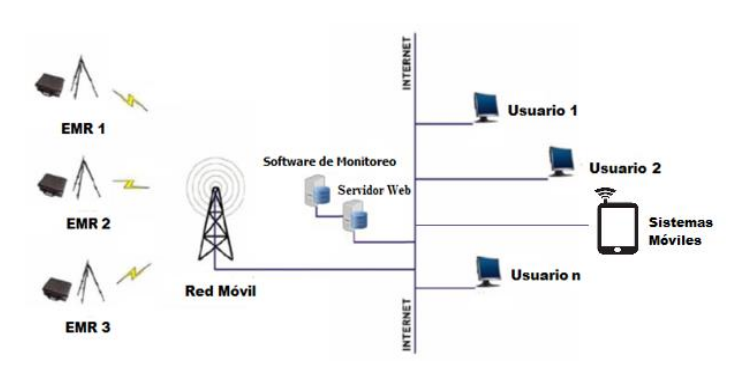
\includegraphics[width=0.6\textwidth]{img/SMI_cartagena.png}
    \caption{Infraestructura típica de un sistema de monitoreo inteligente de ruido. Fuente: \parencite{epacartagena2015}}
    \label{fig:diagrama-sistema-cartagena}
\end{figure}
}{}

\newenvironment{alcances}{El presente proyecto se enfoca en el análisis del ruido generado en el área de los laboratorios del DEI, repasando los apartados vistos en la primera entrega que serán tomados en cuenta para esta segunda etapa del proyecto.

\begin{itemize}
    \item Medición de niveles de ruido: Se utilizarán sensores de sonido conectados a microcontroladores ESP8266 para captar datos acústicos en tiempo real en los diferentes laboratorios del DEI\ para monitorizar los ruidos generados por el alumnado.
    \item Generación de alertas: Cuando los niveles de ruido excedan el umbral permitido, el sistema enviará 
    notificaciones automáticas por correo electrónico. 
    \item Recolección y presentación de datos: Se implementara un servicio que almacenará y procesará los datos de sonido recogidos por los sensores, gestionará la información de reservas y administrará el envío de notificaciones. Asimismo, se desarrollará una interfaz web que permitirá visualizar los niveles de ruido por zona, gestionar configuraciones y consultar registros históricos.
    \item Cobertura de monitoreo: el dispositivo ESP8266 se implementará su instalación en el área de los laboratorios del DEI, el monitoreo empezará a recopilar cuando el laboratorio no se encuentra reservado para su uso. 
\end{itemize}

}{}
\newenvironment{limitaciones}{
El sistema busca ofrecer una solucion efectiva para el monitoreo de ruido en los laboratorios, sin embargo, existen ciertas limitaciones que deben considerarse:

\begin{itemize}
    \item Precisión de los sensores: Al ser sensores de uso educativo, tienen limitantes por ejemplo en la
    calibración, la resolución y la sensibilidad a interferencias de otros ruidos ambientales. 
    \item Dependencia de la API de la universidad: La disponibilidad y estabilidad de la API interna de la
    universidad pueden afectar la obtención de datos en tiempo real sobre la existencia y el estado
    de reservas en las zonas configuradas.
    \item Tiempo de desarrollo: Debido a las limitaciones de tiempo para la ejecución del proyecto,
    se priorizaron las funcionalidades esenciales, dejando mejoras y optimizaciones para futuras
    iteraciones.
\end{itemize}

}{}
\newenvironment{objetivogeneral}{Completar el desarrollo e implementación de un sistema de monitoreo de ruido utilizando la tecnología del Internet de las Cosas (IoT), fusionando el prototipo existente con los servicios de la Universidad Centroamericana "José Simeón Cañas" (UCA), para garantizar funcionalidad plena y capacidad de uso del sistema con el fin de alertar de manera eficiente al personal administrativo sobre altos niveles de ruido en los espacios designados.
}{}
\newenvironment{objetivosespecificos}{
\begin{itemize}
    \item Vincular el dispositivo de monitoreo de ruido de la UCA a los servidores institucionales para el almacenamiento y gestión de datos en tiempo real.
    \item Diseñar y fabricar una carcasa para el dispositivo que asegure durabilidad, practicidad y buen funcionamiento del dispositivo.
    \item Completar la soldadura y el ensamblaje final del prototipo, asegurando que el dispositivo funcione correctamente.
    \item Establecer un sistema de notificaciones vía correos electrónicos a los responsables designados sobre niveles de ruido altos en los espacios designados.
\end{itemize}

}{}

%=================================================================
%                Sección editable para capítulos
% ================================================================
% ================= NO MODIFICAR LOS COMANDOS ====================
% ================================================================

\newcommand{\capitulos}{
    \capitulo{Estuctura de los capítulos}{
    Los capítulos de "introduccion" y "conclusiones y recomendaciones" son obligatorios, pero para el resto de capítulos no existe una estructura obligatoria que se deba seguir y los estudiantes deberan optar por utilizar la estructura que ellos consideren apropiada y que se adapte mejor al tema de su trabajo, sin embargo la universidad recomienda seguir la siguiente estructura:

    \begin{listaenumerada}
        \item Marco teórico
            \begin{enumerate}[label=1.\arabic*]
              \item ¿Que es el ruido?
              \item El impacto de la salud como consecuencia del ruido fuerte
              \item Contaminación sonora y sus consecuencias 
            \end{enumerate}
        \item Metodología
        \item Presentación, análisis e interpretación de resultados
    \end{listaenumerada}
    }
    \capitulo{Marco teórico}{

\begin{enumerate}[label=\textbf{1.\arabic*}]
\item \textbf{¿Qué es el ruido?}\\

El término "ruido" significa simplemente "ruidos molestos". El ruido ambiental incluye, por ejemplo, el ruido del tráfico (vehículos de motor, trenes, aviones), el ruido industrial (máquinas) o el ruido del ocio (gritos fuertes o música, etc.). Sin embargo, la evaluación de la música en particular depende obviamente en gran medida de la percepción subjetiva; si es agradable, se llama "sonido" - de lo contrario "ruido". Dependiendo del país, hay diferentes regulaciones y leyes para regular el ruido ambiental. \\

            
Éstos se diferencian entre distintos niveles, empezando por los ruidos molestos que perturban las actividades humanas o la vida silvestre, aumentan los niveles de estrés o de agresión o conducen a la alta presión sanguínea. En casos extremos, los niveles de ruido muy altos pueden tener efectos negativos duraderos en la salud, como la pérdida de audición, el
tinnitus, los trastornos del sueño, el estrés agudo, los trastornos cardiovasculares o las enfermedades vasculares. En la naturaleza, el ruido provoca un aumento de la tasa de mortalidad tanto en los animales de presa como en los herbívoros debido a una percepción deteriorada, un comportamiento de apareamiento alterado o a la pérdida del sentido de orientación o de la audición.\\
            
\item \textbf{El impacto del ruido fuerte en la salud}\\ 
                    
 La contaminación sónica es uno de los grandes problemas en la sociedad moderna a escala mundial.\\
            
 El reconocimiento del ruido como un peligro para la salud es reciente y sus efectos han pasado a ser considerados un problema sanitario cada vez más importante. Dicha contaminación es la primera causa de contaminación ambiental en Francia, y la segunda en toda Europa. De forma global, Japón es el país más ruidoso del mundo, seguido de España,considerando a Madrid una de las capitales más ruidosas en todo el mundo, según estudios realizados por la OMS.$^[^1^]$ \\
        
El ruido se define como un sonido indeseable, el sonido viaja en forma de ondas en el medio aéreo (o los cambios de presión) lo que produce la vibración del tímpano, el tímpano transfiere estas vibraciones a tres huesos minúsculos en el oído medio,los que a la vez comunican las vibraciones al fluido contenido en la cóclea (en el oído interno) Dentro de la cóclea se hallan las pequeñas terminales nerviosas usualmente conocidas como células ciliadas. Ellas responden a las vibraciones del fluido enviando los impulsos nerviosos al cerebro que entonce interpreta los impulsos como sonido o ruido.$^[^1^]$ \\

            \begin{figure}[h]
              \centering
              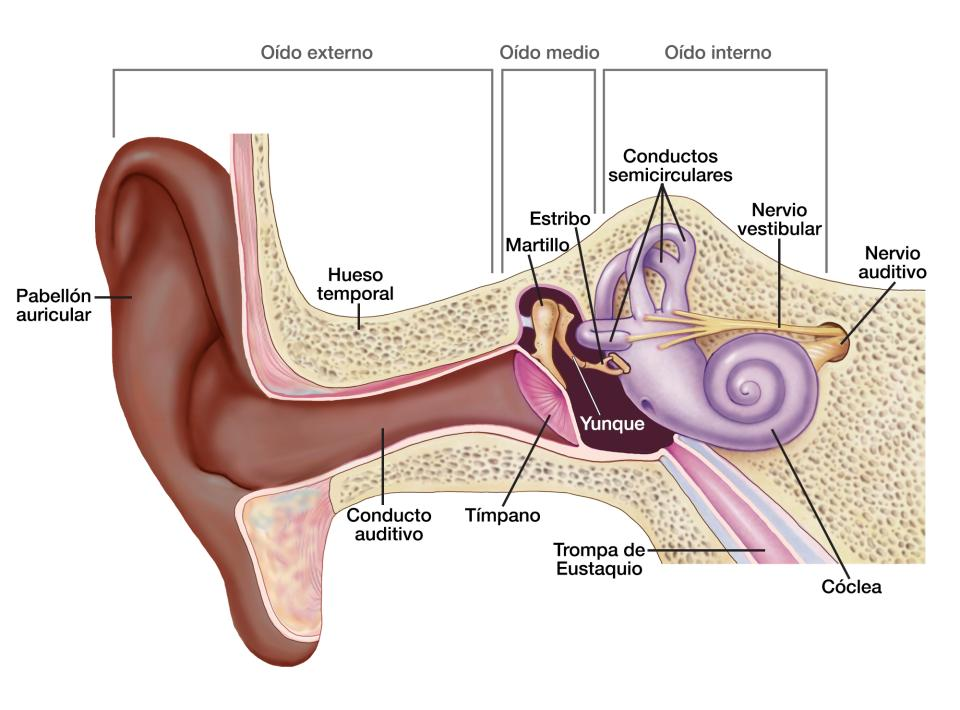
\includegraphics[width=0.7\textwidth]{img/Oido.jpg}
              \caption{Fuente: NIH/NIDCD 2022}
              \label{fig:your_label}
            \end{figure} 
        
 El ruido es considerado un peligro para la salud humana y sus efectos son catalogados como un problema sanitario cada vez más agravante. Puede causar desde insomnio, ansiedad, depresión, estrés, entre otros efectos psicológicos, hasta la pérdida parcial o total de la audición. Un ambiente que sobrepase los 55 decibelios (dB) es considerado un ambiente ruidoso, de 75 a 100dB es considerado un ambiente con ruido fuerte y superior a los 100dB es considerado un ambiente con ruido intolerable.$^[^3^]$ \\

\item \textbf{Contaminación sonora y sus consecuencias} \\

En la investigación previa (fase 1) de este trabajo de graduación se establecieron las bases teóricas sobre el problema que representa la contaminación acústica, cómo se identifica, cuál es el origen o los factores que originan mayormente la contaminación auditiva, estándares internacionales del límite permisible o tolerable para los seres humanos en el estándar de medición de rudio (decibelios) y las consecuencias que trae consigo la contaminación auditiva \parencite{carpio2025}. 
Si ahondamos un poco en el tema, son muchas las consecuencias tanto leves como graves las que se generan por permitir o mantener la contaminación auditiva en un entorno de aprendizaje como lo es el campus UCA   \\

\item \textbf{Efecto del ruido en los estudiantes} \\

Como situación Internacional, una investigación realizada en
2002 por el Doctor Alain Muzet, del Centro de Estudios
Bioclimáticos en Francia, demuestra que los niños cuyos
colegios lindan con zonas ruidosas (industrias, aeropuertos o
carreteras con mucho tránsito) tardan más en aprender a leer,
presentan mayor agresividad, fatiga, son más susceptibles a
peleas y riñas frecuentes, tienen mayor tendencia al
aislamiento, y cierta dificultad de relación con los demás.

        \end{enumerate}
            



    
    }
    \capitulo{Metodología}{
    Descripción de los métodos utilizados para el logro de los objetivos del trabajo.
    }
    \capitulo{Presentación, análisis e interpretación de resultados}{
    En esta sección de debe explicar cómo los resultados se derivan de las mediciones realizadas. Pueden añadirse diagramas para clarificar el diseño experimental, gráficos y tablas para ilustrar mejor los resultados. Por otra parte, en el análisis e interpretación de los resultados se debe responder a la pregunta planteada en la introducción. Es necesario hacer énfasis en porqué sus resultados son relevantes. Finalmente plantee las fortalezas y las debilidades de su estudio.
    }
    \capitulo{Formato de los trabajos}{
    A continuación, se muestran las características principales del formato de trabajos de graduación creado por la facultad de ingeniería y arquitectura de la UCA.
    
    \begin{lista}
        \item \textbf{Partes del documento:}
        \begin{lista}
            \item Primera portada.
            \item Segunda portada.
            \item Agradecimientos (opcional).
            \item Dedicatorias (opcional).
            \item Resumen.
            \item Índice.
            \item Índice de figuras.
            \item Índice de tablas.
            \item Siglas.
            \item Abreviaturas.
            \item Nomenclatura.
            \item Capítulos.
            \item Glosario (opcional).
            \item Referencias.
            \item Anexos.
        \end{lista}

        \item \textbf{Formato general:}
        \begin{lista}
            \item Pagina tamaño carta.
            \item Margen de 2.5cm en todos lados.
            \item Borde de encuadernación de 1cm.
            \item Fuente Times New Roman 11pt.
            \item Interlineado 1.5pt.
            \item Espacio extra entre párrafos 0.
            \item Línea vacía entre párrafos.
            \item Todas las secciones deben comenzar en página impar.
            \item En todas las secciones que llevan título, el titulo se coloca al inicio de la página, en negrita, en mayúscula y centrado horizontalmente.
            \item Debe haber separación de una línea vacía entre el título y el texto.
        \end{lista}

        \item \textbf{Portadas:}
        \begin{lista}
            \item Texto centrado horizontalmente.
            \item Espacio igual entre los párrafos para que el texto ocupe todo el espacio disponible.
            \item Texto en mayúscula.
            \item Fuente tamaño 14pt.
            \item Logo de la primera portada 2.5cm de alto.
            \item En la primera portada los nombres de los integrantes van ordenados en orden alfabético basados en el primer apellido.
    \end{lista}

    \item \textbf{Agradecimientos:}
    \begin{lista}
        \item Extensión máxima una página.
    \end{lista}

    \item \textbf{Dedicatoria:}
    \begin{lista}
        \item Una por cada integrante.
        \item Extensión máxima una página.
        \item Debe llevar el nombre correspondiente del integrante al final de la página y alineado al lado derecho.
    \end{lista}

    \item \textbf{Resumen:}
    \begin{lista}
        \item Extensión de una a tres páginas.
    \end{lista}

    \item \textbf{Índice:}
    \begin{lista}
        \item El espacio horizontal entre el nombre de las secciones y el número de página debe estar lleno de puntos.
        \item Se permite hasta tres niveles de título.
        \item Los títulos de las secciones principales van en mayúscula.
        \item Al final se deben colocarlos anexos.
    \end{lista}

    \item \textbf{Índice de figuras e índice de tablas:}
    \begin{lista}
        \item Cada entrada del índice de figuras debe iniciar con la palabra “Figura” seguido del número de capitulo y el número correlativo de la figura.
        \item Cada entrada del índice de tablas debe iniciar con la palabra “Tabla” seguido del número de capitulo y el número correlativo de la tabla.
    \end{lista}

    \item\textbf{Siglas, abreviaturas y nomenclatura:}
    \begin{lista}
        \item Van separados en dos columnas, en la columna izquierda se coloca la sigla o palabra seguido de dos puntos y en la columna derecha se coloca la definición.
    \end{lista}

    \item\textbf{Figuras:}
    \begin{lista}
        \item Las figuras incluyen gráficos, diagramas, fotos, etc.
        \item El epígrafe va en la parte inferior centrado horizontalmente.
        \item Al inicio va la palabra “Figura” seguido del número de capitulo y número correlativo.
        \item En el epígrafe continuo a la descripción de la figura va la fuente.
        \item La fuente sigue el siguiente formato, “Fuente: [apellido autor, año]”.
        \item Si la figura es de elaboración propia se coloca, “Fuente: [Elaboración propia]”.
        \item Si la figura ha sido adaptada de alguna parte se coloca, “Adaptado de: [apellido autor, año]”.
        \item Las figuras se pueden colocar con orientación horizontal, en ese caso siempre de izquierda a derecha.
        \item Si la figura tiene orientación horizontal, el epígrafe se coloca en el lado derecho de la página.
    \end{lista}

    \item\textbf{Tabla:}
    \begin{lista}
        \item El epígrafe va en la parte superior, centrado horizontalmente.
        \item Al inicio va la palabra “Tabla” seguido del número de capitulo y número correlativo.
        \item La fuente se coloca en la parte inferior, centrada horizontalmente.
        \item La fuente sigue el siguiente formato, “Fuente: [apellido autor, año]”.
        \item Si la tabla es de elaboración propia se coloca, “Fuente: [Elaboración propia]”.
        \item Si la figura ha sido adaptada de alguna parte se coloca, “Adaptado de: [apellido autor, año]”.
        \item Las tablas se pueden colocar con orientación horizontal, en ese caso siempre de izquierda a derecha.
        \item Si la tabla tiene orientación horizontal, el epígrafe se coloca en el lado izquierdo de la página.
    \end{lista}

    \item\textbf{Ecuaciones:}
    \begin{lista}
        \item Las ecuaciones deben estar numeradas de la siguiente forma “(Ec.1.1)”.
    \end{lista}

    \item \textbf{Glosario:}
    \begin{lista}
        \item Tiene el mismo formato que las siglas, abreviaturas y nomenclatura.
    \end{lista}

    \item\textbf{Referencia:}
    
    \begin{lista}
        \item El formato de la referencia es en formato APA.
        \item No se coloca sangría en las líneas de cada una de las referencias.
        \item Las referencias van separadas horizontalmente por una línea vacía.
    \end{lista}

    \begin{itemize}
        \item Álvarez, I. A., Martínez, J. M., Pérez, L. D., Figueroa, F. A., de Armas Mestre, J., & Llop, M. L. R. (2017). Contaminación ambiental por ruido. Revista médica electrónica, 39(3), 640-649.
        \item Gómez, S. S. (2007). Efectos de la contaminación acústica sobre la salud. Revista de salud Ambiental, 7(2), 175-180.
        \item Alfaro-Rojas, D., Portuguez-Brenes, I., Perdomo-Velázquez, H., & Vargas-Masís, R. (2020). Ruido ambiental en áreas verdes urbanas y periurbanas de una microcuenca en Heredia, Costa Rica. Cuadernos de Investigación UNED, 12(2), 419-432.
        \item ¿Qué es el ruido y cómo se puede combatir? (s. f.). https://www.nti-audio.com/es/servicio/conocimientos/-que-es-el-ruido-y-como-se-puede-combatir
        \item Marcelo, Q. G., De Arquitectura Y Urbanismo, F., & De Diseño, E. (2009). El ruido como problema en el aprendizaje: — personalización masiva, modelamiento paramétrico y diseño generativo enfocados al desarrollo de paneles acústicos para salas de clase. https://repositorio.uchile.cl/handle/2250/100197
    \end{itemize}

    \item\textbf{Portada anexos:}
    \begin{lista}
        \item Los anexos se enumeran utilizando letras.
        \item La portada de los anexos lleva dos partes, lleva la palabra “ANEXO” en mayúscula seguido de la letra correspondiente, el tamaño de fuente de esta parte es 20pt.
        \item El título del anexo en mayúscula, el tamaño de fuente de esta parte es 16pt.
        \item Todo el texto va centrado vertical y horizontalmente.
    \end{lista}

    \end{lista}
    }
}

%=================================================================
%       Sección editable para conclusiones y recomendaciones
% ================================================================
% ================= NO MODIFICAR LOS COMANDOS ===================
% ================================================================

\newenvironment{conclusiones}{En esta sección se escriben las conclusiones a las que se ha llegado luego de realizar el trabajo, las conclusiones deben concordar con los objetivos planteados anteriormente.}{}

\newenvironment{recomendaciones}{
En esta sección, se presentan las recomendaciones hechas por el grupo de trabajo para las personas que se beneficiarán del estudio o proyecto realizado.
}{}

%=================================================================
%                Sección editable para glosario
% ================================================================
% ================= NO MODIFICAR LOS COMANDOS ====================
% ================================================================

\newcommand{\mostrarglosario}{true}
\itemglosario{Glosario}{En esta sección, se incluyen términos utilizados en el documento cuya definición podría\newline no ser conocida por el lector, especialmente aquellos de carácter técnico. Esta sección\newline es opcional, como por ejemplo: BackEnd (Parte de una aplicación web que gestiona\newline la lógica, el procesamiento de datos y la comunicación con el servidor).}
\itemglosario{}{}
\itemglosario{}{}



%=================================================================
%                    Sección editable para anexos
% ===============================================================
% ================== NO MODIFICAR LOS COMANDOS ==================
% ================================================================

\newcommand{\anexos}{
    \anexo{anexos}{
     En los anexos se colocan los documentos, gráficos, tablas, imágenes u otros materiales complementarios que proporcionan información adicional relevante, pero que no forman parte del cuerpo principal del trabajo.
    }
}

